A very important feature was for the user to be able to select multiple seats at once. This was especially important, because a venue can have a lot of seats and selecting them one by one would be very time-consuming. A common operation by the user is also moving entire sectors. To tackle this challenge, we decided to develop the multiselect tool. The multiselect tool draws a rectangle when selected and dragged on the map. Everything inside this rectangle is selected. For the rectangle part, Leaflet already provides a feature that uses a rectangle, that works on the drag interaction of the user. This feature is called BoxZoom. The BoxZoom feature is a built-in feature of Leaflet, that allows the user to draw a rectangle on the map and zoom into the area of the rectangle. This feature was a good starting point for the multiselect tool, because it already provides the rectangle drawing and the drag interaction. The BoxZoom feature was extended to provide the multiselect tool. The multiselect tool is a subclass of the BoxZoom feature and overwrites the functions that are responsible for the zooming. Instead of zooming, the multiselect tool selects all the seats inside the rectangle. The multiselect tool is shown in listing \ref{lst:multiselect-tool}. The finished functionality when selecting seats is shown in figure \ref{fig:multiselect-tool}.

\begin{figure}
    \centering
    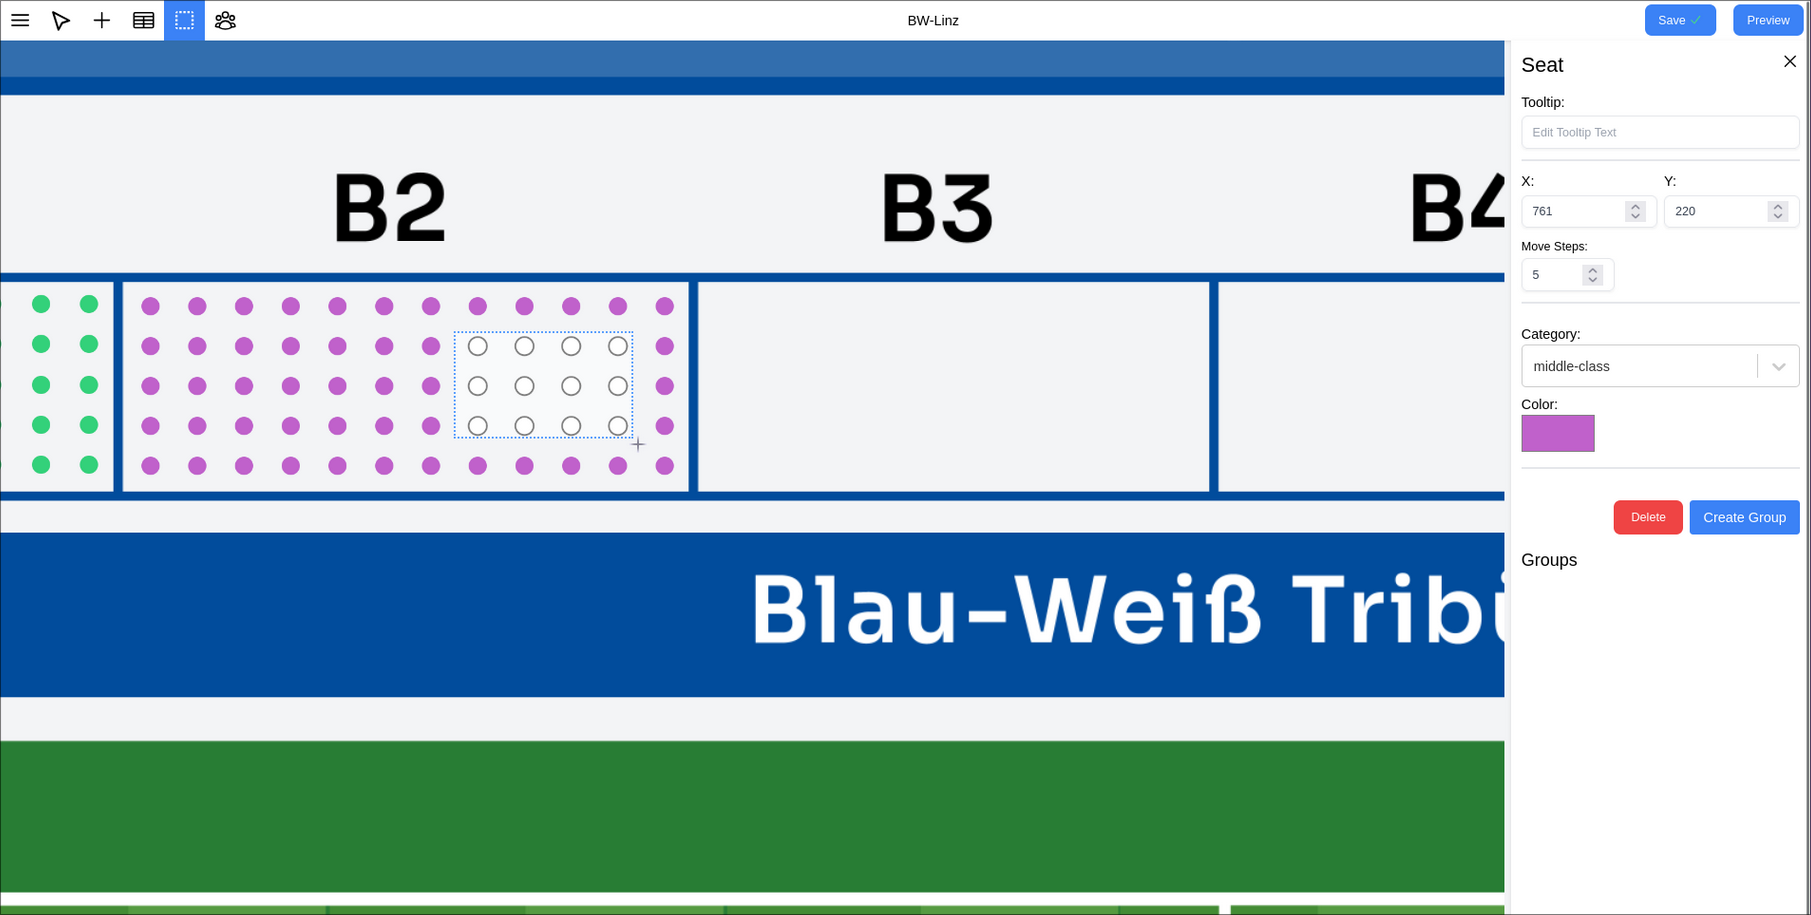
\includegraphics[scale=0.22]{pics/multiselect.png}
    \caption{Multiselect Tool}
    \label{fig:multiselect-tool}
\end{figure}

\begin{lstlisting}[language=Typescript, caption={Multiselect Tool},label={lst:multiselect-tool}]
const MapBoxSelect = (props) => {
    const propsRef = useRef(props);

    useEffect(() => {
        propsRef.current = props;
    }, [props]);

    let _startPoint;
    let _currFunction;

    function checkIfNothingSelected() {
        const currentProps = propsRef.current;
        return (currentProps.currentSelectedTool === undefined || currentProps.currentSelectedTool === null || !(currentProps.currentSelectedTool.id in currentProps.handleDrag));
    }

    L.Map.Multiselect = L.Map.BoxZoom.extend({
        _onMouseDown: function (e) {
            if (checkIfNothingSelected()) {
                return false;
            }
            _currFunction = propsRef.current.handleDrag[propsRef.current.currentSelectedTool.id]
            L.DomUtil.disableTextSelection();
            propsRef.current.mapRef.current?.dragging.disable()

            _startPoint = this._map.mouseEventToLayerPoint(e);

            this._box = L.DomUtil.create('div', 'leaflet-zoom-box', this._pane);
            L.DomUtil.setPosition(this._box, this._startLayerPoint);

            this._container.style.cursor = propsRef.current.currentSelectedTool;

            L.DomEvent
                .on(document, 'mousemove', this._onMouseMove, this)
                .on(document, 'mouseup', this._onMouseUp, this)
                .on(document, 'keydown', this._onKeyDown, this)
                .preventDefault(e);

            this._map.fire('boxzoomstart');
        },

        _onMouseMove: function (e) {
            if (checkIfNothingSelected()) {
                return false;
            }
            var startPoint = _startPoint,
                box = this._box,

                layerPoint = this._map.mouseEventToLayerPoint(e),
                offset = layerPoint.subtract(startPoint),

                newPos = new L.Point(
                    Math.min(layerPoint.x, startPoint.x),
                    Math.min(layerPoint.y, startPoint.y));

            L.DomUtil.setPosition(box, newPos);

            box.style.width = (Math.max(0, Math.abs(offset.x) - 4)) + 'px';
            box.style.height = (Math.max(0, Math.abs(offset.y) - 4)) + 'px';
        },

        _onMouseUp: function (e) {
            if (checkIfNothingSelected()) {
                return false;
            }

            this._finish();
            const map = this._map,
                layerPoint = map.mouseEventToLayerPoint(e);
            const bounds = new L.LatLngBounds(
                map.layerPointToLatLng(layerPoint),
                map.layerPointToLatLng(_startPoint)
            )

            if (_currFunction != null) {
                _currFunction(bounds);
            }
            _currFunction = null
        },

        _finish: function () {
            propsRef.current.mapRef.current?.dragging.enable()
            if (Array.from(this._pane.children).includes(this._box)) {
                this._pane.removeChild(this._box);
            }
            this._container.style.cursor = '';

            L.DomUtil.enableTextSelection();

            L.DomEvent
                .off(document, 'mousemove', this._onMouseMove)
                .off(document, 'mouseup', this._onMouseUp)
                .off(document, 'keydown', this._onKeyDown);
        },

    })

    L.Map.mergeOptions({boxPrinter: true});
    L.Map.addInitHook('addHandler', 'boxPrinter', L.Map.Multiselect);

    L.Map.mergeOptions({boxZoom: false});
}

export default MapBoxSelect
\end{lstlisting}

This code uses parts of the original code concepts, and adapts it for the selecting of seats. 

Except for this tool another way of selecting multiple seats at once was implemented, because of usability reasons, and the expectancy of the user. In editors ranging from Photoshop, Gimp, to File Explorers, the holding of the \texttt{strg} or \texttt{cmd} key while clicking on an object, allows the user to select multiple objects. This was also implemented in SeatGen. The user can hold this key and click on a seat, to select more than one seat.